\chapter{\ifenglish Background Knowledge and Theory\else ทฤษฎีที่เกี่ยวข้อง\fi}

% การทำโครงงาน เริ่มต้นด้วยการศึกษาค้นคว้า ทฤษฎีที่เกี่ยวข้อง หรือ งานวิจัย/โครงงาน ที่เคยมีผู้นำเสนอไว้แล้ว ซึ่งเนื้อหาในบทนี้ก็จะเกี่ยวกับการอธิบายถึงสิ่งที่เกี่ยวข้องกับโครงงาน เพื่อให้ผู้อ่านเข้าใจเนื้อหาในบทถัดๆ ไปได้ง่ายขึ้น
โครงงานนี้ได้นำองค์ความรู้ในด้านของ Computational Intelligence และ การ streaming แบบ Peer-to-peer   
ของรูปภาพจาก application ไปยัง backend ผ่าน WebRTC (Web Real Time Communications) เพื่อให้ backend 
ที่เป็น Computational Intelligence ทำการ classification products โดยโครงสร้างของระบบจะเป็นดังรูป \ref{fig:Overall project structure}
\begin{figure}[h]
  \begin{center}
  % 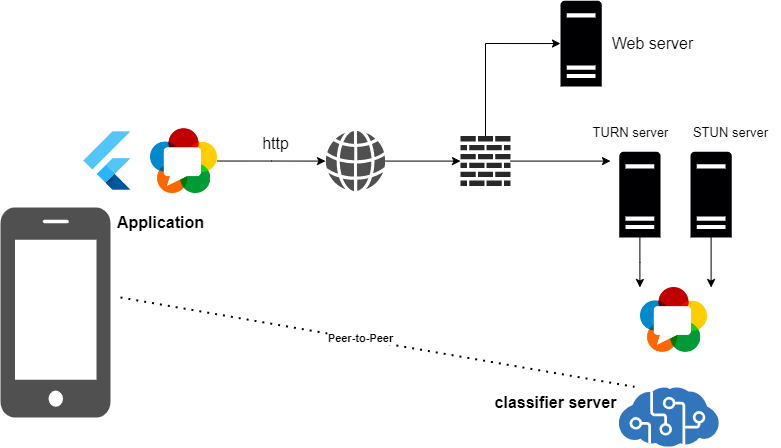
\includegraphics{pic/webrtc.png}
  \vspace{0.5cm}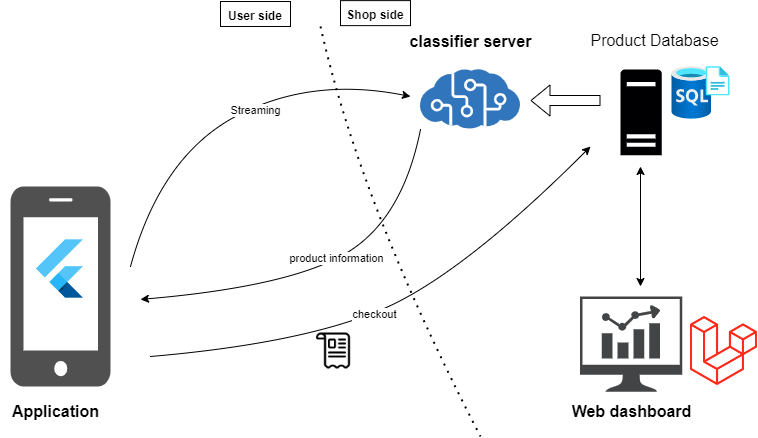
\includegraphics[scale=0.5]{pic/overall.png}
  \end{center}
  
  \caption[Overall project structure]{Overall project structure}
  \label{fig:Overall project structure}
  \end{figure}
  
  \newpage
 
\section{WebRTC for Streaming image}
WebRTC (Web Real-Time Communication) เป็น open-source  ที่ให้บริการ  web browsers
 และ mobile applications ด้วยการสื่อสารแบบเรียลไทม์ (RTC) ผ่าน (API)  
 ทำให้การ Communication ด้วยเสียงและวิดีโอได้ผ่าน  Peer-to-peer   โดยตรงตามรูป \ref{fig:webrtc structure}
 
 
\begin{figure}[h]
\begin{center}
% 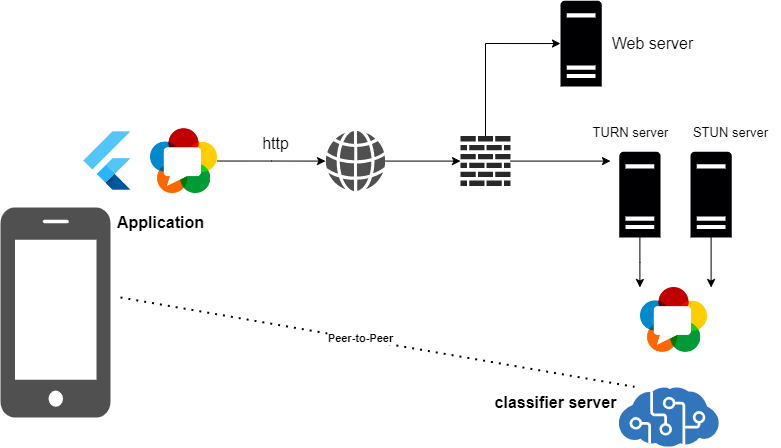
\includegraphics{pic/webrtc.png}
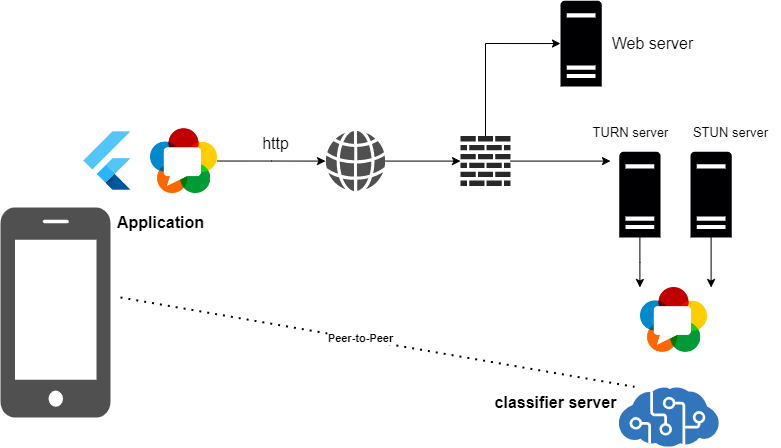
\includegraphics[scale=0.5]{pic/webrtc.png}
\end{center}

\caption[webrtc structure]{webrtc structure}
\label{fig:webrtc structure}
\end{figure}



% \section{Product database}
% Section 2 text.

\section{Transfer Learning}
เป็นเทคนิคที่นำ model ที่ผ่านการฝึกฝนจนแก้ ปัญหาในงานอื่นๆที่มีความคล้ายคลึงกัน
นำมาเป็น model ตั้งต้น สำหรับ model ในการแก้ปัญหาใหม่ๆ
ตัวอย่างเช่น โมเดลที่ได้รับการฝึกฝนให้จดจำวัตถุในภาพสามารถใช้
เพื่อระบุวัตถุที่คล้ายกันในภาพต่างๆ ได้ 
แม้ว่าภาพใหม่จะมีสภาพแสงหรือพื้นหลังต่างกันก็ตาม
 กุญแจสำคัญคือการระบุคุณสมบัติทั่วไปหรือการเป็นตัวแทนที่ใช้ร่วมกันระหว่างโดเมนต้นทางและโดเมนเป้าหมาย
 วิธี Transfer Learning ที่ได้รับความนิยมมากที่สุดวิธีหนึ่งคือ fine-tuning 
คือการใช้โมเดลที่ผ่านการ  pre-trained  มาแล้ว นำมา train ต่อบน ชุดข้อมูลใหม่
และใช้ learning rate น้อยๆ เพื่อป้องกัน weight ที่เคยผ่านการ train จนมีความแม่นยำเปลี่ยนแปลงไปมาก จนไม่มีความแม่นยำ
อีกวิธีหนึ่งคือ feature extraction ซึ่งเกี่ยวข้องกับการใช้ โมเดลที่ผ่านการ  pre-trained  เป็นตัวแยกคุณลักษณะของ ข้อมูล และ สร้าง model ใหม่เพื่อ train จากคุณลักษณะเหล่านี้ที่ model ตั้งต้นแบ่งแยกออกมาได้
 
% \subsection{Transfer Learning}
\begin{figure}[h]
  \begin{center}
  % 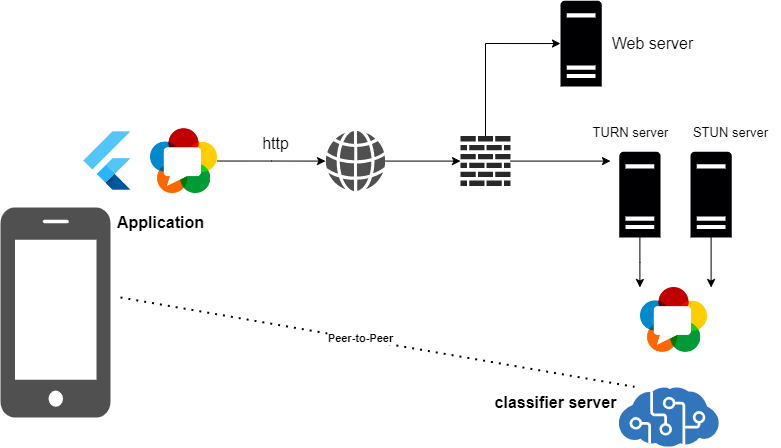
\includegraphics{pic/webrtc.png}
  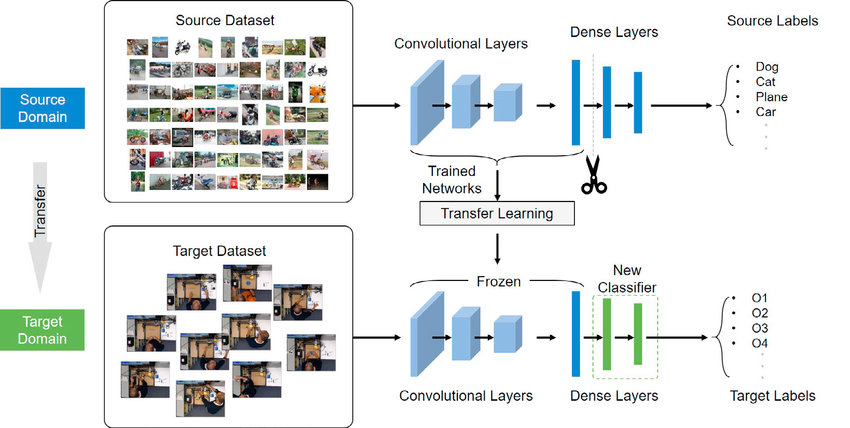
\includegraphics[scale=0.45]{pic/The-architecture-transfer-learning.png}
  \end{center}
  
  \caption[The concept of transfer learning]{The concept of transfer learning}
  \label{fig:The concept of transfer learning}
  \end{figure}
  
% \section{classification products}

% \section{web dashboard}
% Section 3 text. The dielectric constant\index{dielectric constant}
% at the air-metal interface determines
% the resonance shift\index{resonance shift} as absorption or capture occurs
% is shown in Equation~\eqref{eq:dielectric}:

% \begin{equation}\label{eq:dielectric}
% k_1=\frac{\omega}{c({1/\varepsilon_m + 1/\varepsilon_i})^{1/2}}=k_2=\frac{\omega
% \sin(\theta)\varepsilon_\mathit{air}^{1/2}}{c}
% \end{equation}

% \noindent
% where $\omega$ is the frequency of the plasmon, $c$ is the speed of
% light, $\varepsilon_m$ is the dielectric constant of the metal,
% $\varepsilon_i$ is the dielectric constant of neighboring insulator,
% and $\varepsilon_\mathit{air}$ is the dielectric constant of air.

% \section{About using figures in your report}

% define a command that produces some filler text, the lorem ipsum.
% \newcommand{\loremipsum}{
%   \textit{Lorem ipsum dolor sit amet, consectetur adipisicing elit, sed do
%   eiusmod tempor incididunt ut labore et dolore magna aliqua. Ut enim ad
%   minim veniam, quis nostrud exercitation ullamco laboris nisi ut
%   aliquip ex ea commodo consequat. Duis aute irure dolor in
%   reprehenderit in voluptate velit esse cillum dolore eu fugiat nulla
%   pariatur. Excepteur sint occaecat cupidatat non proident, sunt in
%   culpa qui officia deserunt mollit anim id est laborum.}\par}

% \begin{figure}
  % \centering

  % \fbox{
    %  \parbox{.6\textwidth}{\loremipsum}
  % }

  % To include an image in the figure, say myimage.pdf, you could use
  % the following code. Look up the documentation for the package
  % graphicx for more information.
  % \includegraphics[width=\textwidth]{myimage}

  % \caption[Sample figure]{This figure is a sample containing \gls{lorem ipsum},
  % showing you how you can include figures and glossary in your report.
  % You can specify a shorter caption that will appear in the List of Figures.}
  % \label{fig:sample-figure}
% \end{figure}

% Using \verb.\label. and \verb.\ref. commands allows us to refer to
% figures easily. If we can refer to Figures
% \ref{fig:walrus} and \ref{fig:sample-figure} and \ref{fig:webrtc}  by name in the {\LaTeX}
% source code, then we will not need to update the code that refers to it
% even if the placement or ordering of the figures changes.

% \loremipsum\loremipsum

% This code demonstrates how to get a landscape table or figure. It
% uses the package lscape to turn everything but the page number into
% landscape orientation. Everything should be included within an
% \afterpage{ .... } to avoid causing a page break too early.
% \afterpage{
%   \begin{landscape}
%   \begin{table}
%     \caption{Sample landscape table}
%     \label{tab:sample-table}

%     \centering

%     \begin{tabular}{c||c|c}
%         Year & A & B \\
%         \hline\hline
%         1989 & 12 & 23 \\
%         1990 & 4 & 9 \\
%         1991 & 3 & 6 \\
%     \end{tabular}
%   \end{table}
%   \end{landscape}
% }

% \loremipsum\loremipsum\loremipsum

% \section{Overfull hbox}

% When the \verb.semifinal. option is passed to the \verb.cpecmu. document class,
% any line that is longer than the line width, i.e., an overfull hbox, will be
% highlighted with a black solid rule:
% \begin{center}
% \begin{minipage}{2em}
% juxtaposition
% \end{minipage}
% \end{center}

% \section{\ifenglish%
% \ifcpe CPE \else ISNE \fi knowledge used, applied, or integrated in this project
% \else%
% ความรู้ตามหลักสูตรซึ่งถูกนำมาใช้หรือบูรณาการในโครงงาน
% \fi
% }

% อธิบายถึงความรู้ และแนวทางการนำความรู้ต่างๆ ที่ได้เรียนตามหลักสูตร ซึ่งถูกนำมาใช้ในโครงงาน

% \section{\ifenglish%
% Extracurricular knowledge used, applied, or integrated in this project
% \else%
% ความรู้นอกหลักสูตรซึ่งถูกนำมาใช้หรือบูรณาการในโครงงาน
% \fi
% }

% อธิบายถึงความรู้ต่างๆ ที่เรียนรู้ด้วยตนเอง และแนวทางการนำความรู้เหล่านั้นมาใช้ในโครงงาน
